\subsection{\FirstTimeDefine{\ProgramGraph}{\ProgramGraphEN}} 

สำหรับโปรแกรมเขียนด้วยภาษาที่มีข้อกำหนดจัดเจนแล้ว {\ProgramGraph}\ คือ \FirstTimeDefine{\DirectedGraph}{\DirectedGraphEN} 
ซึ่งแต่ละ {\FirstTimeDefine{\Node}{\NodeEN}} แทนส่วนประกอบของชุดคำสั่ง โดย{\FirstTimeDefine{\Edge}{\EdgeEN}} แทนการไหลของการควบคุม 
หาก $i$ และ $j$ คือ {\Node}ในกราฟโปรแกรม ที่เชื่อมกันด้วย{\Edge}แบบมีทิศทางจาก $i$ ไปยัง $j$ แล้ว จะสื่อความหมายว่า 
"{\Node} $j$ จะทำงานในลำดับถัดไปหลังจากที่ $i$ ทำงานเสร็จสิ้น" \cite{Jorgensen2013} โดยเริ่มต้นด้วย{\Node}ที่มีดีกรีออก 
(Outdegree) มีค่าเป็น 1 และสิ้นสุด ณ \Node ที่มีดีกรีเข้า (Indegree) มีค่าเป็น 1 เช่นเดียวกัน ซึ่งรูปแบบความสัมพันธ์ของกราฟโปรแกรมนั้น 
McCabe \cite{Watson1996} ได้กำหนดรูปแบบโครงสร้างการทำงานขั้นพื้นฐานของการพัฒนาโปรแกรม 
(The primitive operations of structured programming) \figpageref{fig:graphtype}

\begin{figure}[ht!]
    \centering
    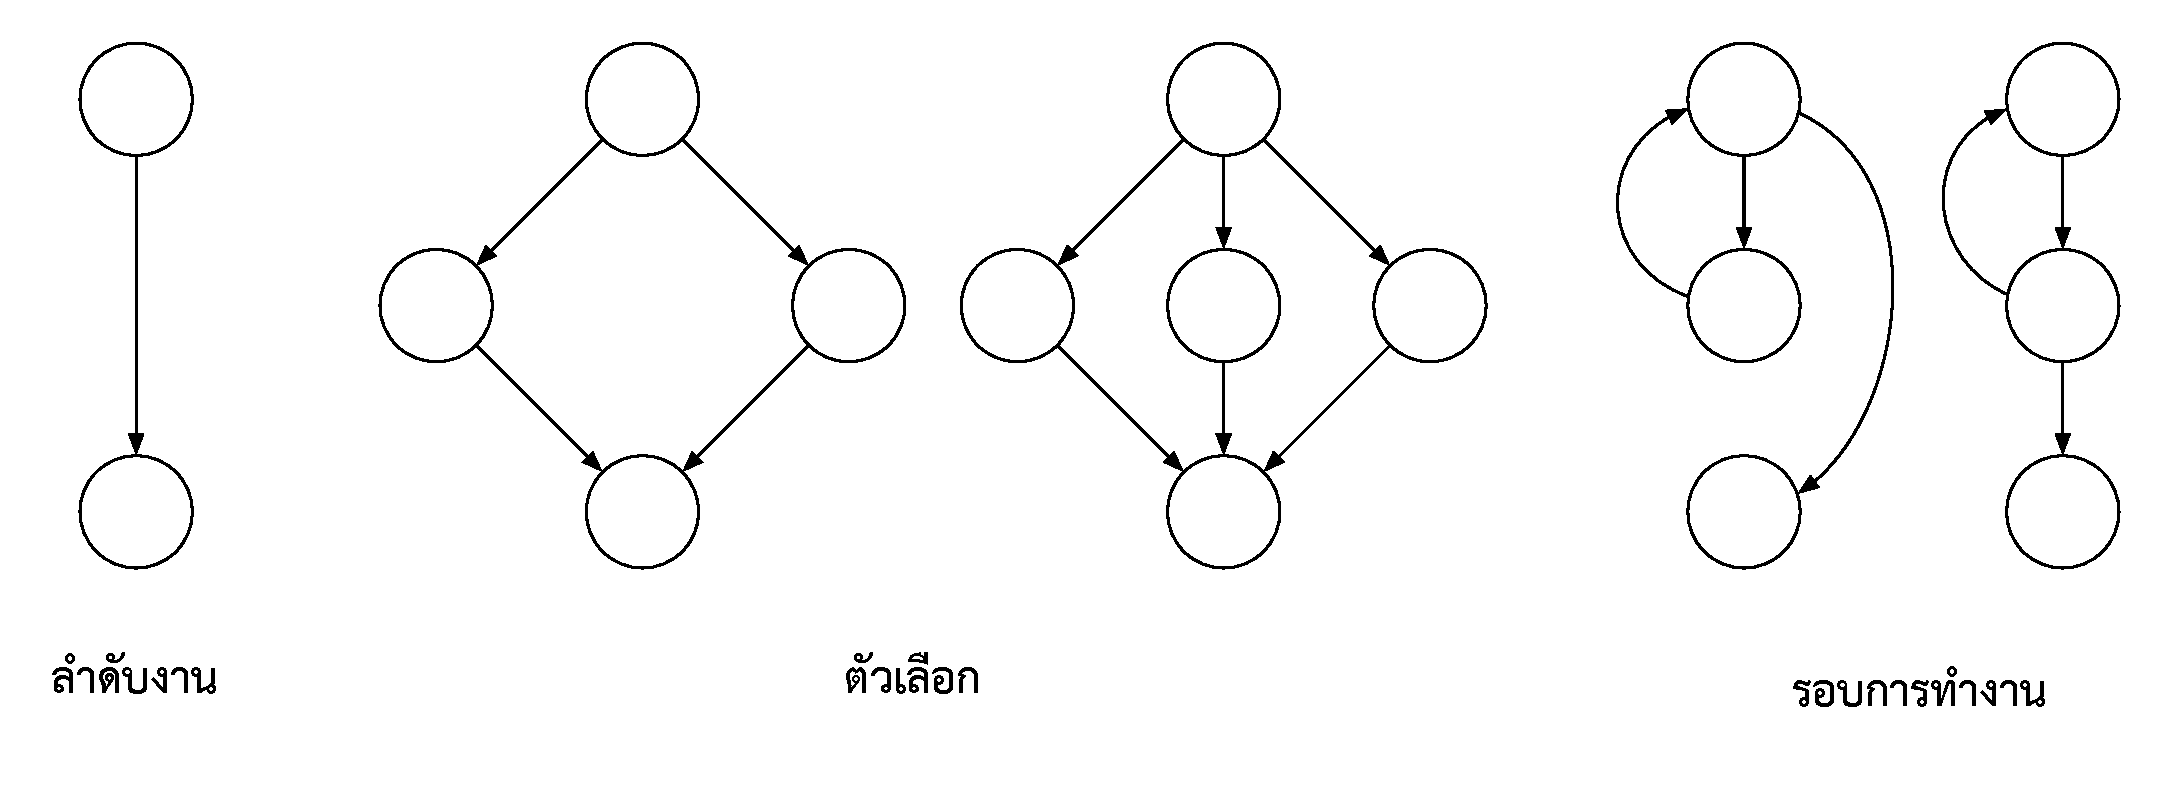
\includegraphics[width=0.9\textwidth]{graph-types}
    \caption{ประเภทของกราฟ}
    \label{fig:graphtype}
\end{figure}

จาก{\figurename} \ref{fig:pseudocodeGrading} (\pagename\ \pageref{fig:pseudocodeGrading}) 
เป็นชุดรหัสเทียมที่นำเสนอวิธีการคำนวณเกรดของนิสิตโดยรับข้อมูล โดยรับข้อมูลคะแนน (student\_score) และคะแนนพิเศษ (bonus\_score) 
ของนิสิต หากมีคะแนนเป็น 0 จะได้เกรด \emph{{\bf I}} หากนิสิตได้คะแนนต่ำกว่า 80 คะแนน จะได้เกรด {\emph{\bf U}} หากมีคะแนนตั้งแต่ 80 
ไปจนถึง 100 คะแนน นิสิตจะได้เกรด {\emph{\bf S}} 

\begin{figure}[ht!]
    \begin{algorithm}[H]
        \begin{algorithmic}[1]
            \STATE{Program {\bf "Simple Grading"}}
            \STATE{student\_score $\gets$ receive student score}
            \STATE{bonus\_score $\gets$ receive student's bonus score}

            \IF{bonus\_score > 0 \AND student\_score <= 50} 
                \STATE{student\_score = min(50, student\_score + bonus\_score)} 
            \ELSIF{bonus\_score > 0 \AND student\_score <= 70} 
                \STATE{student\_score = min(70, student\_score + bonus\_score)}
            \ENDIF

            \STATE{grade\_letter = ""}

            \IF{student\_score < 80} 
                \STATE{grade\_letter = 'U'} 
            \ELSIF{student\_score == 0}
                \STATE{grade\_letter = 'I'} 
            \ELSIF{student\_score <= 100}
                \STATE{grade\_letter = 'S'} 
            \ENDIF

            \STATE{print(grade\_letter)}
        \end{algorithmic}
    \end{algorithm}
    \caption{ชุดรหัสเทียมสำหรับคำนวณเกรดนิสิตจากคะแนนที่ได้รับ}
    \label{fig:pseudocodeGrading}
\end{figure}

จากชุดรหัสเทียมข้างต้นสามารถแปลงเป็นกราฟโปรแกรม เพื่อทำความเข้าใจโครงสร้างได้ดัง{\figpageref{fig:programGraph} 

\begin{figure}[hbt!]
    \centering
    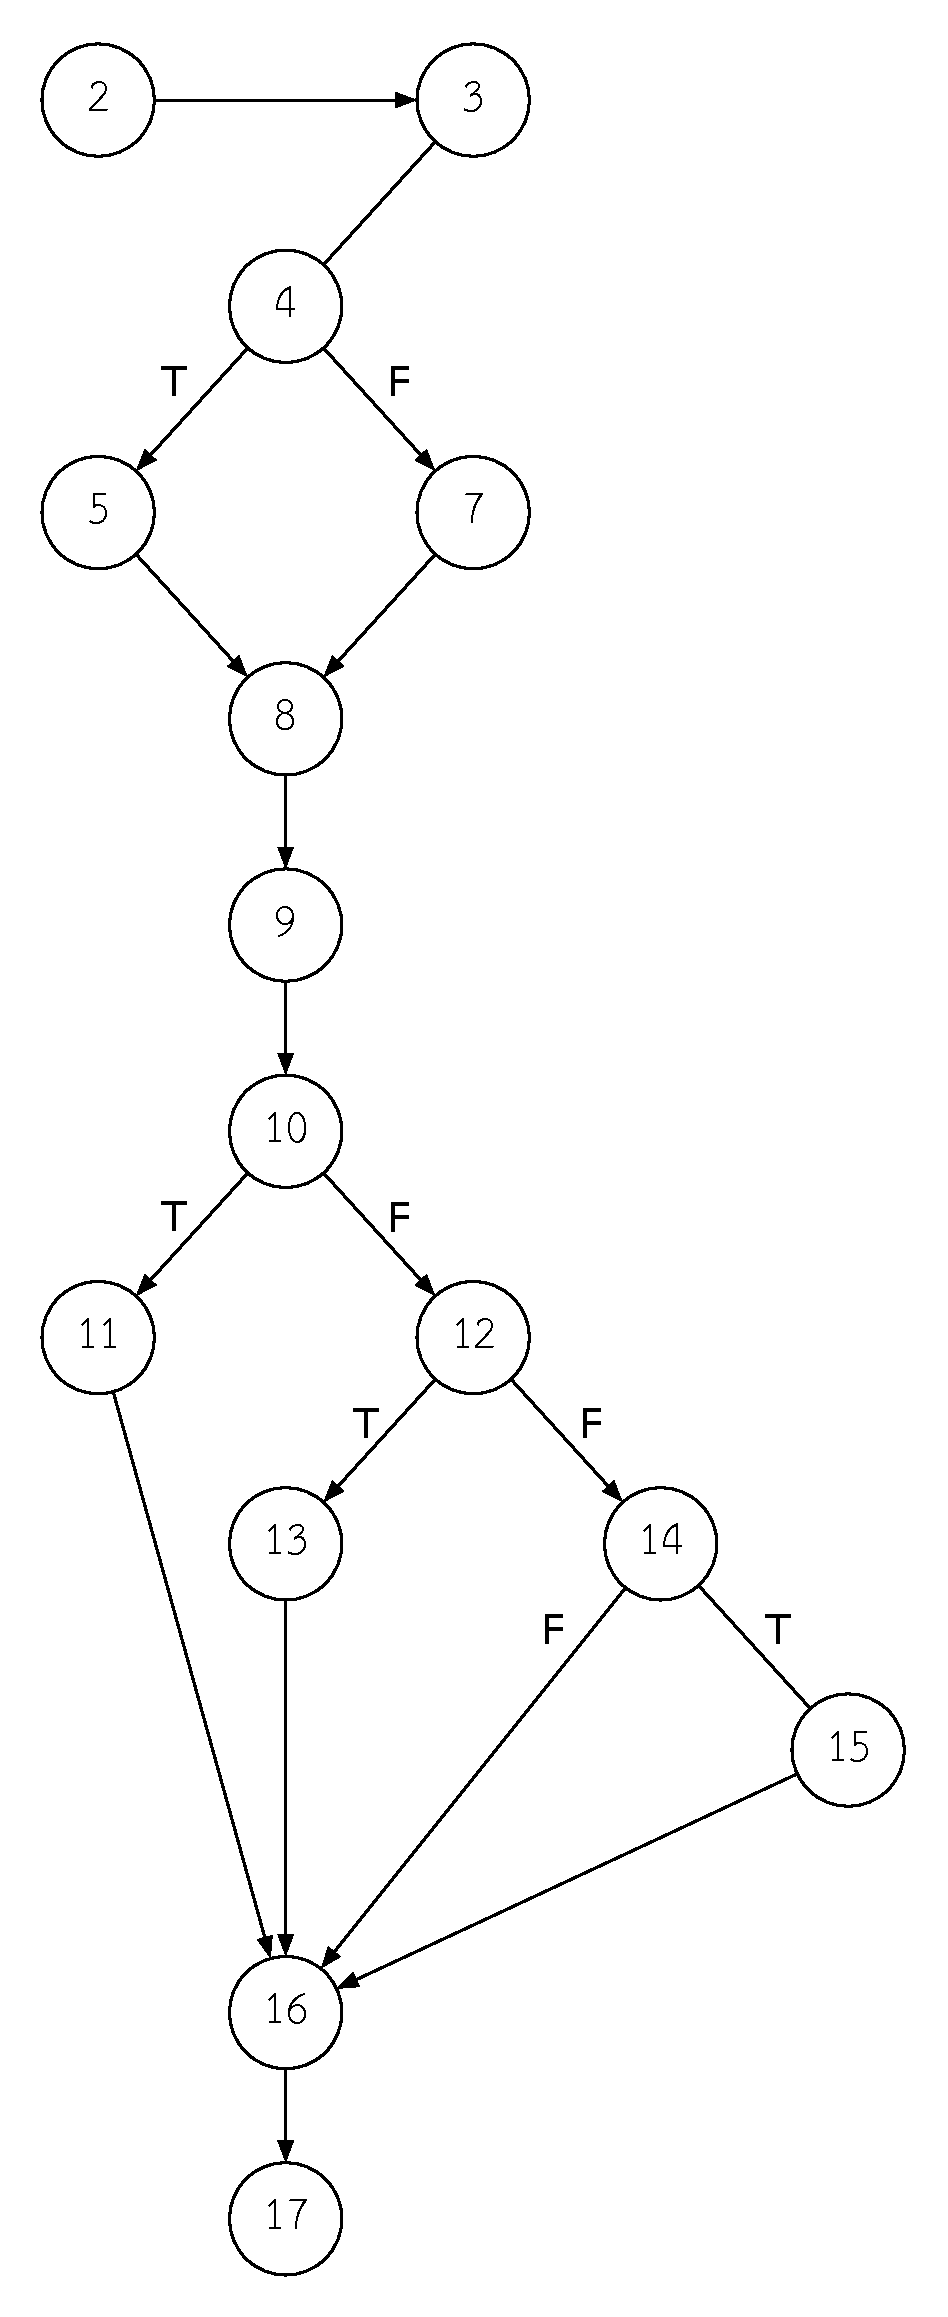
\includegraphics[height=0.65\textheight]{grading-program-graph}
    \caption{กราฟโปรแกรมของชุดรหัสเทียมสำหรับคำนวณเกรดนิสิต}
    \label{fig:programGraph}
\end{figure}

จาก{\figurename} \ref{fig:programGraph} (\pagename\ \pageref{fig:programGraph}) เป็นการนำเสนอชุดรหัสเทียบจาก
{\figref{fig:pseudocodeGrading} ในรูปของกราฟโปรแกรม โดยที่{\Node}ที่ 2-3, 7, 9, 11, 13, 15 และ 16 
คือ{\Node}ที่แสดงถึงลำดับการดำเนินงาน และ{\Node} 4, 6, 10, 12 และ 14 
เป็น{\FirstTimeDefine{\PredicateNode}{\PredicateNodeEN}} ภายในโปรแกรม โดยมีโหนด 2 และ 17 
เป็น{\FirstTimeDefine{\sourcenode}{\sourcenodeEN}} และ{\FirstTimeDefine{\sinknode}{\sinknodeEN}}\ ตามลำดับ 

การนำเสนอโปรแกรมในรูปของกราฟโปรแกรมนั้นช่วยให้ผู้ทดสอบวิเคราะห์โครงสร้างของโปรแกรมจากกราฟ 
เพื่อหาข้อผิดพลาดในโครงสร้างของโปรแกรมง่ายขึ้น ด้วยการแยก{\FirstTimeDefine{\BasisPath}{\BasisPathEN}} 
จากกราฟข้างต้น โดยแต่ละ{\BasisPath}ที่แยกนั้นจะเริ่มต้นด้วย{\sourcenode} และสิ้นสุดด้วย{\sinknode}เดียวกัน 
จากนั้นจึงเลือก{\BasisPath}ที่ต้องการทดสอบเป็น \FirstTimeDefine{\TestPath}{\TestPathEN} จากนั้นจึงวิเคราะห์{\PredicateNode}
ที่ปรากฎบน{\TestPath} พิจารณาเงื่อนไข แล้วจึงสร้างกรณีทดสอบพร้อมทั้งข้อมูลทดสอบตามวิธีการที่ผู้ทดสอบเห็นสมควร 
ซึ่งจะได้กรณีทดสอบที่ทำให้โปรแกรมดำเนินการบน{\TestPath} ที่เลือกมาได้ ยกตัวอย่างเช่น 
หากเลือก{\BasisPath}จาก{\figref{fig:programGraph}} เป็น{\TestPath} จะพบว่ามี{\PredicateNode}บน{\TestPath}ด้วยกัน 2 {\Node} 
ด้วยกัน ได้แก่ {\bf 4} และ {\bf 10} เมื่อพิจารณา{\PredicateNode}ทั้ง 2 จะได้ข้อมูลทดสอบเป็น {\bf bonus\_score = 1} และ 
{\bf student\_score = 50} ซึ่งข้อมูลทดสอบที่สร้างขึ้นนี้สามารถทำให้โปรแกรมทำงานใน{\TestPath}ได้ 
ดังกรณีทดสอบใน\tabref{tab:simpleTestCase}

\begin{figure}[ht!]
    \centering
    \small{$2\ \textendash\ 3\ \textendash\ 
                (4)\ \textendash\ 5\ \textendash\ 8\ \textendash\ 9\ \textendash\ 
                (10)\ \textendash\ 11\ \textendash\ 16\ \textendash\ 17$}
    \caption{ตัวอย่าง{\TestPath}สำหรับโปรแกรมคำนวณเกรด}
    \label{fig:testpath}
\end{figure}


\begin{table}[ht!]
    \centering
    \caption{กรณีทดสอบ}
    \label{tab:simpleTestCase}
    \begin{tabular}{|l|c|c|c|}
    \hline
    \rowcolor{LightGray}
    Case ID     & bonus\_score  & student\_score    & Expected output \\
    \hline
    SC1         & 1             & 50                & U \\
    \hline
    \end{tabular}
\end{table}

\subsection{\FirstTimeDefine{\scg}{\scgEN}}

การพัฒนาโปรแกรมเชิงวัตถุ (Object-oriented programing: OOP) คือการจำลองพฤติกรรมและความสามารถจากชีวิตจริงออกมาเป็น
{\FirstTimeDefine{\class}{\classEN}} \FirstTimeDefine{\method}{\methodEN} 
และ{\FirstTimeDefine{\attribute}{\attributeEN}} \cite{kindler2011} ซึ่งโปรแกรมใด
โปรแกรมหนึ่งที่พัฒนาขึ้นด้วยแนวคิดการพัฒนาเชิงวัตถุ นั่นคือการดำเนินงานสอดประสานร่วมกันของ{\class}ผ่าน{\method} 
ดังนั้นเพื่อให้เข้าใจถึงความสัมพันธ์กันระหว่าง{\sourcecode} ด้วย{\scg} โดยที่แต่ละ{\Node}แทน{\class} 
หากคลาสเรียกใช้งาน{\method}ของ{\class}อื่น ตัวอย่างเช่น หากแปลงชุดรหัสเทียมจาก \figpageref{fig:pseudocodeGrading} 
เป็น{\sourcecode}ภาษาจาวา (Java) ตามแนวคิดเชิงวัตถุ 
% ด้วยแนวคิดพื้นฐานของออกแบบเชิงวัตถุ (Object-oriented design) \cite{Martin2016} นิยามไว้โดย Robert C. Martin 
% ซึ่งเป็นแนวคิดการออกแบบที่นักพัฒนานำไปใช้งานโดยทั่วไป 
โดยแยกออกเป็น 2 \class\ ได้แก่ \code{SimpleBonusScore} และ \code{SimpleGrading} ดัง \figpageref{fig:javaBonusScore}
และ\figpageref{fig:javaGrading}ตามลำดับ

\begin{figure}[ht!]
    \lstset{style=thesiscodestyle}
    \lstinputlisting[language=Java]{related/SimpleBonusScore.java}
    \caption{{\sourcecode}ภาษาจาวาสำหรับคำนวนคะแนนเพิ่มพิเศษ}
    \label{fig:javaBonusScore}
\end{figure}

\begin{figure}[ht!]
    \lstset{style=thesiscodestyle}
    \lstinputlisting[language=Java]{related/SimpleGrading.java}
    \caption{{\sourcecode}ภาษาจาวาสำหรับคำนวณเกรดนิสิต}
    \label{fig:javaGrading}
\end{figure}


% - - - - - - - - - - - - - - - - - - - -
\clearpage
จาก\figpageref{fig:javaGrading} เมื่อกำหนดให้ \code{G} แทน{\class} \code{SimpleGrading} และ \code{B} 
แทน\class\ \code{SimpleBonusScore} โดยที่\class\ \code{SimpleGrading} เรียกใช้งาน{\method} \code{score} 
ซึ่งเป็น{\method}ของ{\class} \code{SimpleBonusScore} ผ่าน{\method} {\code{grading}} ดังนั้น{\scg}สำหรับความสัมพันธ์นี้จะเป็นดัง
{\figpageref{fig:subscggrading}} ซึ่งในการพัฒนาจริงนั้น\class\ \code{SimpleGrading} และ\class\ \code{SimpleBonusScore}
อาจมีการเรียกใช้งานระหว่างกันมากกว่า 1 \method ดังที่ได้แสดงใน{\figpageref{fig:subactualscg}}

\begin{figure}
    \begin{minipage}[t]{0.5\linewidth}
        \centering
        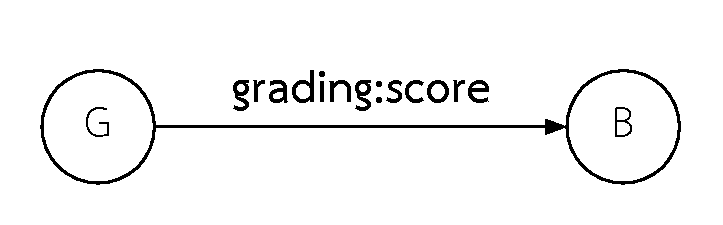
\includegraphics[width=0.8\textwidth]{simple-static-call-graph}
        \subcaption{{\scg}โปรแกรมคำนวณเกรดนิสิต}
        \label{fig:subscggrading}
    \end{minipage}%
    \begin{minipage}[t]{0.5\linewidth}
        \centering
        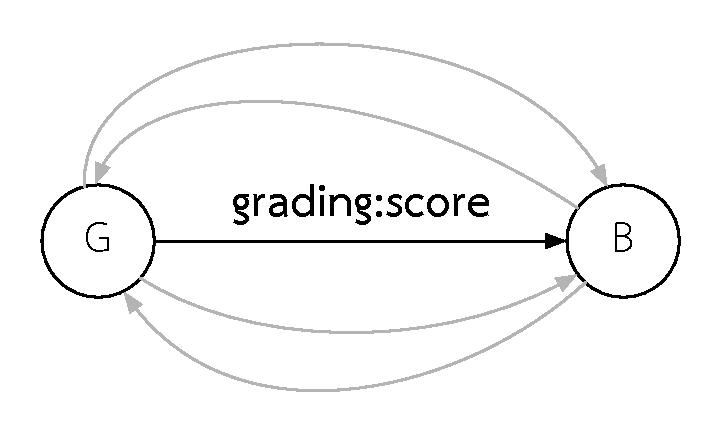
\includegraphics[width=0.8\textwidth]{simple-static-call-graph-multiple-call}
        \subcaption{{\scg}ของโปรแกรมในกรณีที่\code{SimpleGrading} มีการเรียกใช้งาน{\code{SimpleBonusScore}} หลาย{\method}}
        \label{fig:subactualscg}
    \end{minipage}%
    \caption{{\scg}โปรแกรมคำนวณเกรดนิสิต}
    \label{fig:scggrading}
\end{figure}

\subsection{\FirstTimeDefine{\InfeasiblePath}{\InfeasiblePathEN}}

\InfeasiblePath คือ ทางเดินที่ไม่สามารถหาค่าทุก ๆ ความเป็นไปได้ซึ่งสอดคล้องกับ{\PredicateNode}ที่อยู่บนทางเดินนั้น 
เพื่อทำให้โปรแกรมทำงานบนเส้นทางนั้นได้ \cite{Naik2008} หากพิจารณาจากชุดรหัสเทียบใน{\figpageref{fig:programGraph}} 
และ{\figpageref{fig:programGraph}} ประกอบเข้าด้วยกัน จะพบว่าทางเดิน 
\code{\overline{10}\ \textendash\ 12\ \textendash\ 13} คือ {\bf \InfeasiblePath} เนื่องจากไม่สามารถหาค่าที่สอดคล้อง
กับ\PredicateNode\ 10 และ 12 นั่นคือ \code{student\_score \geq 80} และ \code{student\_score = 0} ได้ในทุก ๆ กรณี

\subsection{\FirstTimeDefine{\Cyclomatic}{\CyclomaticEN}}

% การวัดความซับซ้อนของโปรแกรมนั้นสามารถทำได้หลายแนวทาง ทั้งการประมาณการจากจำนวนกรณีทดสอบ 
% ที่ครอบคลุม{\sourcecode}ได้ตามระดับความครอบคลุม (Coverage level) \cite{Ferrer2013} ตามที่ต้องการ
% หรือประเมินความซับซ้อนของแผนภาพกระบวนการทางธุรกิจ (Business Process Model and Notation: BPMN) ที่จะนำโปรแกรมเข้าไปช่วยบริหารจัดการ
% \cite{Solichah2013}
ในการวัดความซับซ้อนเชิงโครงสร้างของโปรแกรมนั้น McCabe ได้กำหนด \Cyclomatic\ \cite{McCabe1976}\ 
ไว้เพื่อเป็นมาตรวัดความซับซ้อนของโปรแกรม โดยใช้การพิจารณาจากจำนวน\Node\ \Edge และ\PredicateNode\ ที่ประกอบกันภายใน\ProgramGraph\ 
ดัง\eq{eq:complexitymeasureStronglyConnected} และ \eq{eq:complexitymeasure}

\begin{align}
    v(G) &= e - n + p \label{eq:complexitymeasureStronglyConnected} \\
    v(G) &= e - n + 2p \label{eq:complexitymeasure} 
\end{align}

\begin{table}[ht!]
    \begin{tabular}{lcl}
    เมื่อ & $v(G)$    & คือ ค่า{\Cyclomatic}ที่คำนวณได้               \\
        & $e$       & คือ จำนวน{\Edge}ใน\ProgramGraph            \\
        & $n$       & คือ จำนวน{\Node}ใน\ProgramGraph            \\
        & $p$       & คือ จำนวนพื้นที่ที่เชื่อมต่อกันใน\ProgramGraph   \\
    \end{tabular}
\end{table}

โดยที่ \eq{eq:complexitymeasureStronglyConnected} จะใช้กับกราฟที่เชื่อมต่อกันแบบเข้ม (Strongly connected graph) 
นั่นคือกราฟนั้นจะต้องมีทางเดินจาก $n_j$ ไปยัง $n_k$ เสมอ แต่หากไม่ใช่แล้วจะใช้ \eq{eq:complexitymeasure} โดยจะกำหนดให้ 
$p = 1$ จาก{\ProgramGraph}ใน{\figpageref{fig:programGraph}} ซึ่งมี{\Edge} ทั้งสิ้น 20 เส้น และจำนวน{\Node}ทั้งสิ้น 
16 \Node ดังนั้นหากคำนวนระดับความซับซ้อนตาม{\Cyclomatic}ของ{\ProgramGraph}นี้ จะได้ว่า

\begin{align*}
    v(G) &= e - n + 2p \\
         &= 19 - 16 + 2(4) \\
    v(G) &= 11
\end{align*}
